\usetikzlibrary{positioning,fit,matrix}
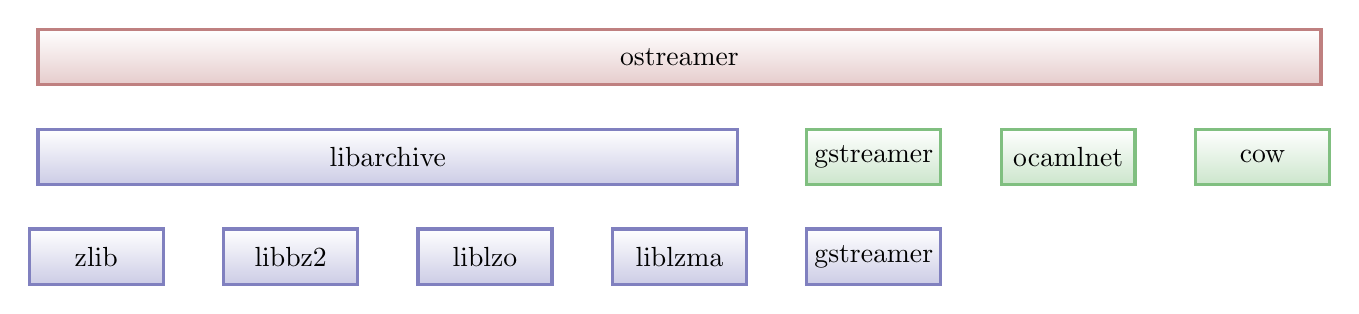
\begin{tikzpicture}[
  redblock/.style={
    rectangle,
    very thick,
    draw=red!50!black!50,
    top color=white,
    bottom color=red!50!black!20,
    inner sep=0em,
    minimum width=17mm,
    minimum height=2em
  },
 blueblock/.style={
    rectangle,
    very thick,
    draw=blue!50!black!50,
    top color=white,
    bottom color=blue!50!black!20,
    inner sep=0em,
    minimum width=17mm,
    minimum height=2em
  },
 greenblock/.style={
    rectangle,
    very thick,
    draw=green!50!black!50,
    top color=white,
    bottom color=green!50!black!20,
    inner sep=0em,
    minimum width=17mm,
    minimum height=2em
  }]
  \matrix (table) [
    %draw
    matrix of nodes,
    nodes in empty cells,
    row sep = 4mm,
    column sep = 10mm,
   nodes={text centered}] {
   & & & & & & & & & & & & & \\
   \\
   & & & & & & & & & & & & & \\
   \\
   & & & & & & & & & & & & & \\
   };
  \node[fit=(table-1-1)(table-1-14),redblock,label={center:ostreamer}]{};
  \node[fit=(table-3-1)(table-3-8),blueblock,label={center:libarchive}] {};
  \node[fit=(table-3-9)(table-3-10),greenblock,label={center:gstreamer}] {};
  \node[fit=(table-3-11)(table-3-12),greenblock,label={center:ocamlnet}] {};
  \node[fit=(table-3-13)(table-3-14),greenblock,label={center:cow}] {};
  \node[fit=(table-5-1)(table-5-2),blueblock,label={center:zlib}] {};
  \node[fit=(table-5-3)(table-5-4),blueblock,label={center:libbz2}] {};
  \node[fit=(table-5-5)(table-5-6),blueblock,label={center:liblzo}] {};
  \node[fit=(table-5-7)(table-5-8),blueblock,label={center:liblzma}] {};
  \node[fit=(table-5-9)(table-5-10),blueblock,label={center:gstreamer}] {};
  \begin{scope}
  %\draw[->,very thick] (table-1-1) -- (table-3-2);
  \end{scope}
\end{tikzpicture}
% http://tex.stackexchange.com/questions/94343/matrix-of-nodes-over-multiple-columns-in-tikz